\documentclass[a4paper,11pt]{report}
\usepackage[T1]{fontenc}
\usepackage[english,ngerman]{babel}
\usepackage[utf8]{inputenc}
\usepackage{titlesec}
\usepackage[onehalfspacing]{setspace}
\usepackage[autostyle=true]{csquotes}
\usepackage{geometry}
\usepackage{fancyhdr}
\usepackage[
  backend=bibtex,
  style=authoryear,
  firstinits=true,
  uniquename=init,
  sortlocale=de_DE
]
{biblatex}
\usepackage{graphicx}
\graphicspath{ {./appendix/} }
\DeclareNameAlias{sortname}{last-first}
\DeclareFieldFormat*{title}{#1}
\DefineBibliographyStrings{ngerman}{
   andothers = {{et\,al\adddot}},            
}
\addbibresource{ref.bib}
\geometry{
  left=25mm,
  right=35mm,
  top=20mm,
  bottom=15mm,
  bindingoffset=5mm
}
\titleformat{\chapter}[display]
  {\normalfont\bfseries}{}{0pt}{\Large}
\titlespacing{\chapter}{0pt}{5pt}{10pt}

\renewcommand{\rmdefault}{phv} % Arial
\renewcommand{\sfdefault}{phv} % Arial
\renewcommand{\headrulewidth}{0.1pt} 
\interfootnotelinepenalty=10000

\usepackage{etoolbox}
\makeatletter
\patchcmd{\chapter}{\if@openright\cleardoublepage\else\clearpage\fi}{}{}{}
\makeatother

\begin{document}
\title{Wurden die richtigen Lehren aus der
    Weltfinanzkrise 2007-2009 gezogen?}
\author{%
    Facharbeit im Leistungskurs Sozialwissenschaften \\
    Ravensberger-Gymnasium Herford \\ \\
    \textit{eingereicht bei} \\
    Herrn Visser \\ \\
    \textit{vorgelegt von} \\
    Gabriel de Souza Tomitsuka 
    }
\date{Herford, Oktober 2019}
\maketitle
\cleardoublepage
\pagenumbering{gobble}
\tableofcontents
\cleardoublepage
\pagenumbering{arabic}
\chapter{Einleitung}
\section{Themenwahl}
Laut dem Gesch\"aftsf\"uhrer der Investmentbank J.P. Morgan
Chase Jamie Dimon sei die Woche des 15. Oktobers 2008, also ab dem
Tag an dem Lehman Brothers Insolvenz anmeldeten, von einer finanzwirtschaftlichen
Perspektive mit der Woche des \enquote{Great Crashes} ab dem 24. Oktober 1929 vergleichbar gewesen, allerdings habe die rechtzeitige Reaktion der Regierungen und
Regulatoren das Schlimmste vermieden \parencite{dimonyt}.
Diese Ansicht teilt auch der ehemalige Gouverneur der Federal
Reserve Bank of New York Geithner, laut dem man knapp eine
Weltwirtschaftskrise vermieden habe, in der Geldautomaten
nicht funktionieren und Tafel deutlich vergr\"oßert werden
m\"ussen \parencite{geithneryt}.

Ich habe mich oft gefragt, wie ein Markt, der
von kleinen, amerikanischen Regionalbanken mit
staatlicher Unterstützung
dominiert wird, zum Fall von als \enquote{Too Big To
Fail} verstandene Investmentbanken wie Lehman
Brothers und Merill Lynch
führen konnte. Besonders interessant fand ich,
dass auch Banken in anderen Kontinenten (wie
bspw. die Dresdner Bank) dadurch
aufgekauft werden mussten.

Ich wollte genauer
ermitteln, wie genau sowas passieren konnte
bzw. heute noch m\"oglich ist, und ob
die Maßnahmen der Beteiligten
womöglich eine noch schlimmere Krise
vermieden haben -- also ob die Behauptung Dimons
und Geithners stimmt.

\section{Vorgehensweise}
Die Ursachen für die Finanzkrise 2008 können 
in zwei Gruppen unterteilt werden: Ursachen der Immobilienkrise
in den Vereinigten Staaten und die finanzwirtschaftlichen
Ursachen der globalen Finanzkrise.

\"Uber die realwirtschaftlichen Ursachen besteht weithin
Einigkeit innerhalb der Wirtschaftswissenschaften, daher
werde ich verk\"urzt auf sie eingehen.

Um die finanzwirtschaftliche Ursachen zu erläutern, werde
ich erst auf die theoretische Grundlage des Finanzsystems
vor und nach den Deregulierungen ab 1980 Jahren eingehen,
sowie die der Bankentheorie. Daraufhin werde ich Verbriefungen
und finanzielle Innovation untersuchen, und wie genau sie für die
Krise mitverantwortlich sind. Ferner werde ich
die Frage erörtern, ob es andere Instrumente
oder Anlageklassen gibt, die eine
besondere Wirkung auf die Krise hatten, welche den
Weg in die \"Offentlichkeit nicht fand.

Daraufhin werde ich die kurzfristige Reaktion
der Regulatoren und Zentralbanker ab 2008
untersuchen (wie bspw. die kontroverse
Bankenrettung). Zus\"atzlich werde ich auf die mittel- und
langfristigen Maßnahmen, mit besonderem Schwerpunkt auf Basel
III eingehen.

Schließlich werde ich mit Bezug auf
unterschiedliche Perspektiven
erörtern, ob diese Maßnahmen die globale
Wirtschaft ausreichend auf die
Herausforderungen der Zukunft vorbereiten,
und ob eine Finanzkrise dieser Ausmaße noch m\"oglich ist.

\chapter{Amerikanische Immobilienkrise}
Über die realwirtschaftlichen Ursachen der Krise besteht
weithin Einigkeit in den Wirtschaftswissenschaften: 
der Kreditboom in den USA und die Immobilienblase.
Im Folgenden werde ich erläutern, wie diese entstanden
sind und wie sie zur Krise beigetragen haben.

\section{Der Hypothekenmarkt}
Aus den f\"unfundsiebzig Millionen H\"ausern im
Privateigentum 2007 in den USA, wurden auf etwa f\"unfzig Millionen
Hypotheken aufgenommen (Buffett, 2018).
In der Zeit zwischen 2002 und 2007 hat sich das
Schulden zu Nationaleinkommen-Verhältnis
der USA von 3,75:1 auf 4,75:1 erhöht.
Um die letzte Erhöhung der Schulden in
dieser Größenordnung zu erreichen, hat man davor
das gesamte Jahrzehnt der 1990er
gebraucht \parencite[S. 195f.]{acharyar}.

Durch das Schaubild in Appendix 1 wird deutlich,
dass das Wachstum der Immobilienpreise keine Verbindung
mit den finanziellen Zugewinnen der Amerikaner hatte,
und zumeist spekulativ war. 

Laut dem US-amerikanischen
Großinvestor Warren Buffett war die Erwartungshaltung
des durchschnittlichen amerikanischen
B\"urgers zu der Zeit,
dass die Immobilienpreise weiterhin rapide ansteigen w\"urden,
und entsprechend dieser Haltung \"uber die Immobilie
gesicherte Kredite aufgenommen haben (Buffett, 2018).

\subsection{Der Subprime-Markt}
Viele Immobilienkredite wurden von Menschen, die sich selbst
in einer Niedrigzinsumgebung die Immobilie nicht leisten
k\"onnten, erworben.
Dazu kommen die strategischen Anreize, um Kreditnehmer
mit wenig Bonit\"at (Subprime) anzuwerben. Dazu z\"ahlen
Kredite ohne Einkommensbeweise (siehe Appendix II), 
und hybride Kredite mit Teaserraten. Sie wurden in "2/28\"\-- oder
"3/27\"\--Modellen verkauft, die sehr attraktive, fixe Zinsraten
f\"ur die ersten zwei bzw. drei Jahre anboten, und
f\"ur die letzten 28 bzw. 27 exorbitant hohe Zinss\"atze\footnote{
  wie solche Kredite m\"oglich waren, wird in 3.3 erl\"aurtert}.
Diese waren so konstruiert, dass sie in ausgesprochen vielen
F\"allen den Kreditnehmer zur Insolvenz f\"uhrten --
es sei denn die Immobilienpreise stiegen deutlich
und er war in der Lage es neu zu finanzieren
\parencite[S. 208]{acharyar}.

Unter diesen Umst\"anden wird deutlich, dass diese eine
Umgebung war, in welcher selbst eine verringerte Wachstumsrate
der Immobilienpreise ausgereicht h\"atte,
um dem Binnenmarkt in den USA zu schaden.

\section{R\"uckgang ab 2006}
Durch sinkende Wachstumsraten und den Anstieg des Leitzinses
auf 5,25\% im Juni 2006 gab es eine Wende.
Die Wachstumsrate des realen HPI (House Price Index,
Purchase Only) sank ab Anfang 2006 und
ab November sank der HPI selbst (Appendix 3).

In August 2006 ist der Anteil der insolventen
Immobilien, die an Subprime Kreditnehmer verkauft wurden,
auf 7.74\% gestiegen (vgl. August 2005: 5,53\%).

Kurz daraufhin waren die ersten spezialisierten
Kreditgeber im Bereich Subprime ebenfalls insolvent - 
Ownit Mortgage Solutions Inc. beantragte im Dezember 2006 Chapter 11
Bankruptcy Protection\footnote{Demnach kann eine insolvente
Firma eine Sanierung bzw. Reorganisation vorschlagen,
um ihre Kredite versp\"atet zahlen zu k\"onnen, und somit
das Gesch\"aft zu retten. In Ownits Fall war dieser Plan nicht
erfolgreich.}. Ownit war derzeit der elftgrößte Kreditgeber
im Subprime-Sektor \parencite{wsjdoss}.

Am 12. M\"arz 2007 h\"orte der zweitgr\"oßte Kreditgeber im Bereich
Subprime, New Century Financial Corporation, auf, neue
Kredite zu geben. Sie meldeten einen Monat sp\"ater Insolvenz 
an\footnote{Die Insolvenz hatte unterschiedliche Gr\"unde -
zus\"atzlich fand New Century keine Investoren mehr
und sie verloren mehrere Sammelklagen.}. 2006 vergaben sie noch
etwa 60 Milliarden Dollar an Krediten \parencite{nytcres}.

Subprime-Kreditnehmer, die hybride Kredite
gekauft haben, wollten zu dieser Zeit ihre Kredite neu finanzieren.
Allerdings war eine Refinanzierung nach dem
Wertverlust der Immobilie sinnfrei. Dies  f\"uhrte zu
einer Welle von Insolvenzen.
Die durchschnittliche amerikanische Familie, dessen Haus
hypothekarisch belastet war und etwa 35\% ihres
Gesamtverm\"ogens betrug, konsumierte im Jahre 2008
aus diesen Gr\"unden deutlich weniger als in den
Vorjahren -- eine Rezession war zu erwarten. 
\parencite[196]{acharyar}

\chapter{Globale Finanzkrise}
Warum diese Faktoren aber zu einer Finanzkrise gef\"uhrt haben,
durch die viele der gr\"oßten Finanzinstitutionen
der Welt gefallen sind und Kapitalm\"arkte eingefroren sind,
ist allerdings viel weniger klar. Um zu verstehen, warum das System
versagt hat, muss man erst verstehen, wie das System aufgebaut war.

\section{Die alte Finanzarchitektur}
Nach der Weltwirtschaftskrise 1929 war die mehrheitlich
vertretene politische Meinung, dass unregulierte
Finanzm\"arkte intrinisisch instabil seien und stark reguliert
werden m\"ussten, um schwere wirtschaftliche Krisen
und politische bzw. gesellschaftliche
Unruhe zu vermeiden. \parencite[S. 563f.]{crottycam}.

Das Bretton-Woods-System,
entwickelt nach den Vorstellungen von John Maynard Keynes
und Harry Dexter White, setzte eine neue globale W\"ahrungs-
und Handelsordnung in Kraft, welche Regierungseingriffe
in W\"ahrungs- und Finanzkrisen erleichtern sollte.

Durch die IMF und die Weltbank sollten Liquidit\"atsprobleme
vermieden werden und Regierungen und Regulatoren langfristig handlungsf\"ahiger werden
\parencite[S. 31f.]{bordo}.

\section{Die neue Finanzarchitektur}
Wirtschaftliche Turbulenzen in den 1970er Jahren f\"uhrten
zu einem Paradigmenwechsel, n\"amlich die \"Uberzeugung, dass staatliche
Vorschriften im Finanzsektor mehr Schaden als Nutzen anrichten.
Im Laufe der Zeit ersetzte die neoklassische Theorie den 
Keynesianismus und die enge regulatorische Umgebung wurde gelockert
-- Geschäftsbanken sollten wenig reguliert werden, Investmentbanken
noch weniger und Schattenbanken (bspw. Hedge- und Private-Equity-Fonds) kaum.

Die Maßnahmen der Deregulierung in den USA fingen im Jahre 1980 an. Der
\textit{Depository Institutions Deregulation and Monetary Control Act (DIDMCA)}
entfernte die Zinsobergrenze und erteilte Banken und anderen
finanziellen Institutionen die Erlaubnis, Darlehen mit variablen
 Zinsen zu vergeben\footnote{Wegen DIDMCA k\"onnen bis heute
 Institutionen, die Kurzzeitkredite an Subprime-Kreditnehmer
 vergeben, Zinss\"atze bis 700\% im Jahr zu verlangen.}
\parencite[6--8]{sherman2009short}.

Zwar ver\"anderte DIDMCA die Dynamik des Kreditmarktes in Amerika
nachhaltig, allerdings war die einflussreichste Deregulierungsmaßname
die Lockerung und anschließende Aufhebung des
\textit{Glass-Steagall Act of 1933}.
Die gesetzliche Trennung von Geschäfts- und Investment-Banken
beabsichtigte eine Vermeidung von Interessenkonflikten und 
\"uberm\"aßiger Risikobereitschaft durch Geschäftsbanken.
In der Praxis bedeutete das, dass eine Gesch\"aftsbank keine 
Verbriefungen b\"urgen oder verkaufen konnte und ausschließlich
erstklassige Wertpapiere f\"ur sich kaufen konnte.

Im Jahre 1986 interpretierte die \textit{Federal Reserve} Glass-Steagall neu:
Geschäftsbanken durften bis zu 5\% ihres Umsatzes durch Investmentbanking
erwirtschaften.

Im Jahre 1996 ging die \textit{Federal Reserve} einen Schritt weiter:
Bankholdinggesellschaften durften bis zu 25\% ihres Umsatzes durch
Investmentbanking generieren, was Glass-Steagall in der Praxis aufhebt,
da nahezu alle Institutionen unter der 25\%-Grenze blieben.

Im Jahre 1999 hob die Clinton-Regierung Glass-Steagall offiziell auf.

Ein weiterer Schritt war die \textit{
  Riegle-Neal  Interstate  Banking  and  Branching Efficiency Act}, die
die Restriktionen des Bankings \"uber die Grenzen eines US-Bundesstaats
entfernt hat. Durch Fusionen sank die Zahl der amerikanischen 
Banken um 27\% zwischen 1990 und 1998 \parencite[8--12]{sherman2009short}.

\subsection{Strukturelle Probleme}
Der postkeynesische \"Okonom James Crotty behauptet, die neue Finanzstruktur
habe auch in der Theorie Probleme. Ein Hauptargument der Neoklassik sei, dass
Kapitalm\"arkte Wertpapiere richtig bepreisen w\"urden und das Risiko gut einsch\"atzen
k\"onnten. Marktteilnehmer seien dementsprechend in der Lage,
richtige Entscheidungen entsprechend ihres Risikoprofils zu treffen.
Somit seien Finanzkrisen sehr unwahrscheinlich, da Marktteilnehmer nur so viel
Risiko aufnehmen w\"urden, wie sie tragen k\"onnen. Allerdings soll dieses Argument
keine empirischen Beweise haben und auf unrealistischen Annahmen basieren
\parencite[563--565]{crottycam}.

\section{Banking in der Theorie und Praxis}
Die klassische Theorie des Bankings ist, dass Banken als Vermittler
zwischen Anleger und Kreditnehmer agieren. Kreditgeber legen ihr Geld
in der Bank an und erwirtschaften damit Zinsen, w\"ahrend die Banken die
Bonit\"at der m\"oglichen Kreditnehmer evaluieren und basierend
auf diesen Evaluationen entleihen.

Dadurch, dass das Geld der Kreditgeber angelegt wird, kann nicht jeder
Kreditgeber sein Geld zum gleichen Zeitpunkt zur\"uckfordern, obwohl er
in den meisten F\"allen einen Anspruch darauf hat -- Um dieses Risiko
zu vermeiden, werden Einlagen bis zu einem bestimmten Niveau durch
die Regierung gesichert (in den USA 100 Tausend Dollar, in der EU 100 Tausend Euro).

Im Gegenzug erwarten Regierungen, dass Banken bestimmte Kapitalpuffer
bereithalten. Zu dem Zeitpunkt der Krise betrug dieser mindestens 8 Prozent\footnote{
  Diese Zahl wird durch die Bank für Internationalen Zahlungsausgleich
  festgelegt. Mitglieder sind nahezu alle Industrienationen und viele
  weitere Entwicklungsl\"ander.
} des Kapitals der Bank \parencite[197--198]{acharyar}.

Dies ist aus Bankenperspektive \"außerst teuer,
es gibt aber einen Ausweg.

\subsection{Verbriefungen}
Im amerikanischen Bankensystem waren im Jahre 2008 etwa 7 Billionen US-Dollar
in Form von Einlagen und etwa 14 Billionen
US-Dollar in Form von Krediten\footnote{
  Davon waren \$1,3 Billionen Subprime-Hypotheken, \$3,3 Billionen kommerzielle
  Hypotheken und \$5.8 Billionen Prime-Hypotheken.} angelegt.
Der Grund f\"ur diese Diskrepanz sind Verbriefungen --
durch sie sind Banken nicht mehr nur Vermittler
zwischen Einleger und Kreditnehmer, sondern zwischen
\textit{Investor} und Kreditnehmer.

Im Gegensatz zu Anlegern brauchen Investoren klare
Zahlungsstr\"ome und m\"ussen wissen, wo und wie 
ihr Geld investiert wird. Außerdem muss
das genaue Risiko eingestuft werden -- diese Zust\"andigkeit
wurde den Ratingagenturen wie Fitch Ratings, Moody's und S\&P
abgegeben.

\textit{Mortgage-Backed Securities (MBS)} sind 
heute noch die beliebteste Form von Verbriefungen.
Sie bestehen aus den Geldfl\"ussen
von Zins- und Tilgungszahlungen
mehrerer Tausend Hypotheken. Sie sind mit zwei
Risiken verbunden: eine Fr\"uhtilgung
oder die Insolvenz des Kreditnehmers.
Etwa 55\% Amerikanische Immobilien waren im Jahre
2008 verbrieft.

In diesem Rahmen sind die Geb\"uhren, die Banken
durch Verbriefungen verdienen, zu einer
Haupteinnahmequelle der Banken geworden. Da eine
Bank durch das Verkaufen einer Verbriefung
das Risiko an eine andere Person oder Institution
\"ubertr\"agt, braucht sie keine Kapitalpuffer.

Ein Vorteil ist, dass dieses Risiko bei fehlerfreier Anwendung
so aufgeteilt ist, dass diese nicht auf eine Institution
konzentriert ist, sondern auf viele Marktteilnehmer,
die nur so viel Risiko aufnehmen, wie sie tragen k\"onnen.
Das reduziert das allgemeine systematische Risiko \parencite[198--201]{acharyar}.
Allerdings gibt es auch große Probleme.

\subsection{Falsche Anreize}
Durch die \"Ubertragung des Risikos werden
viele falsche Anreize f\"ur Vermittler geschaffen. 
Das l\"asst sich leicht am Beispiel der Subprime-Hypotheken aufzeigen.
Wie in Abbildung 2 ersichtlich, sahen viele
Hypothekenspezialisten und -banken keinen Grund, die 
Bonit\"at ihrer Kunden zu \"uberpr\"ufen, da die Hypotheken
unabh\"angig davon an eine große Bank verkauft werden konnten.
Demnach war die Kommission unabh\"angig vom langfristigen Erfolg
der Immobilie \parencite[565]{crottycam}.

Die Investmentbanken schufen ebenfalls falsche Anreize.
Die Formel zur Berechnung der Boni ber\"ucksichtigte ausschließlich
die sofortigen Gewinne bzw. Verluste durch die Bildung und den Verkauf
der Verbriefungen.
Die mittel- und langfristigen Folgen f\"ur die Bank
spielten hierbei keine Rolle.
Merill Lynch, die Investmentbank, die im Rahmen der Finanzkrise von
Bank of America aufgekauft werden musste um eine Insolvenz zu umgehen,
dient hier als gutes Beispiel. Sie sch\"utteten im Jahre 2008 \$3.6
Milliarden an Boni aus,
obwohl die Bank \$27 Milliarden im selben Jahr verlor\footnote{genug, um fast zehn Jahre an Profiten \enquote{auszugleichen}} \parencite[565]{crottycam}.

Kreditratingagenturen spielten eine große Rolle, da
die Größe der Kapitalpuffer
von dem Rating der Anlagen abh\"angig ist.
Dadurch, dass die Kredite in Triple-A-Wertpapiere
verpackt waren, mussten Banken deutlich weniger Kapitalpuffer bereithalten
 -- im System nach Basel II brauchte ein Triple-A-Wertpapier
 nur die H\"alfte des Kapitalpuffers eines klassischen Kredits.

Investmentbanken machten von der M\"oglichkeit, die
Ratingagentur selbst auszusuchen, Gebrauch. Wenn die Ratings
einer Agentur schlechter als erhofft ausfielen, wurde die Agentur gewechselt.

Zus\"atzlich erm\"oglichte ein Triple-A-Rating
den Verkauf an Institutionen wie Geldmarktfonds,
die gesetzlich dazu
verpflichtet sind, haupts\"achlich in die sichersten Wertpapiere
zu investieren. Da diese Fonds grunds\"atzlich
wenige besonders profitable Investitionsm\"oglichkeiten haben,
waren f\"ur sie indirekte Investitionen in CDOs
besonders attraktiv. Diese geschahen \"uber
\textit{Asset-Backed Commercial Paper} (ABCP), welche h\"aufig
r\"uckblickend ignoriert werden.

Diese waren f\"ur Banken sehr risikoreich,
da Geldmarktfonds nur kurzfristig Kapital
liehen -- Banken mussten ihre ABCPs regelm\"aßig erneuern.
Sie verwendeten \emph{kurzfristig} geliehenes Kapital
um \emph{langfristige} illiquide Wertpapiere
zu finanzieren \parencite[201]{acharyar}.

Banken machten von dieser Strategie Gebrauch, um Verbriefungskommissionen
zu erh\"ohen, was in den Boomjahren \"außerst profitabel war.
Als sich die Lage auf dem Subprime-Kreditmarkt aber verschlechterte,
entschieden sich diese Fonds, ihre Investition nicht zu erneuern.
Da Investmentbanken f\"ur die Wertpapiere in den ABCPs hafteten,
mussten diese zu Lasten der Banken nun mit der Bilanz verrechnet
werden. Ungef\"ahr \$400 Milliarden
in Form von Verbriefungen erreichten dadurch
im Jahre 2008 die Bilanzen globaler Banken \parencite[570]{crottycam}.

Im Interview behauptet der H\"andler T. Rossi, dass dieser Aspekt
zum Fall von Lehman Brothers und Merill Lynch gef\"uhrt habe.
Diese Banken hatten in k\"urzester Zeit Hunderte
Milliarden mehr an Verbindlichkeiten zu bilanzieren, ohne im Besitz entsprechender
Liquidit\"at zu sein. Das f\"uhrte dazu, dass ihre \textit{
  Capital Adequacy Ratio
} (CAR), also das Verh\"altnis von Kapital zu Assets, aus der
Perspektive der Regulatoren nicht ausreichend war und viele Banken
gleichzeitig gezwungen wurden, risikoreichere Positionen massenhaft zu liquidieren,
was wiederrum zu noch mehr Angst in den Kapitalm\"arkten f\"uhrte.

Dadurch mussten Banken in wenigen Monaten
mehr Kapital auftreiben, als das Eigenkapital der
Bank betrug (siehe Appendix: Interview 3).
Die wenigsten Investoren waren \"uberhaupt in der Lage,
die ben\"otigte Liquidit\"at den Banken zuzuf\"uhren.

Wenige Investmentbanken wie J.P. Morgan 
verringerten schon 2006/07 ihr Risiko im Immobilienmarkt
und fingen an, Kapital aufzutreiben \parencite{dimonyt}.

Allerdings waren viele Banken bem\"uht, bis Ende von
der Immobilienblase zu profitieren\footnote{
  CEO der Citigroup in 2007: \foreignquote{english}{When
    the music stops, in terms of liquidity, things will be complicated.
    But as long as the music is playing, you've got to get up and dance.
    We're still dancing}
}, was sie ihre finanzielle Lage drastisch verschlechterte,
sodass ihre einzigen Optionen die Insolvenz oder die Rettung
durch die Regierung waren (siehe Appendix: Interview 3).

\section{Finanzielle Innovation und strukturierte Produkte}
Finanzielle Innovation ist f\"ur strukturierte
Kreditprodukte verantwortlich, die so komplex sind, dass sie
zwangsl\"aufig intransparent sind. Dementsprechend
kann die Theorie des fairen Preises durch den Markt 
auf komplexe strukturierte Produkte nicht angewandt werden \parencite{crottycam}.

Eine hypothekenbesicherte CDO (Collateralized Debt 
Obligation) besteht aus bis zu 150 MBS.
Eine CDO wird in viele
Tranchen aufgeteilt (daher strukturiert),
abh\"angig vom Grad des Risikos.
Die Mezzanine-Tranchen
sind risikoreicher, da sie als erste Verluste
erleiden -- daf\"ur haben sie viel h\"ohere Zinsen.
Erst wenn die Mezzanine-Tranchen wertlos sind,
kommen Verluste bei den Seniortranchen an.

Eine \textit{CDO-Squared} (besondere Art der Verbriefungen zweiter Stufe)
ist eine CDO, die Tranchen vieler CDOs als Sicherungsgegenst\"ande verwendet.
Es ist nahezu unm\"oglich, eine CDO-Squared fair zu bepreisen.
Das liegt teilweise
daran, dass die selbe MBS in mehreren CDOs vorkommen kann \parencite[224--226]{chackocred}.

Diese Komplexit\"at missbrauchten Banken um bessere Ratings f\"ur ihre
Mezzanine-Tranchen zu sichern. Eine CDO-Squared mit haupts\"achlich
Mezzanine-Tranchen und wenigen Senior-Tranchen konnte f\"ur mehr
verkauft werden, als die Summe ihrer Teile einzeln wert waren
\parencite[26--28]{iwregulation}.

Laut Prof. Dr. George Chacko der Harvard Business School gibt es kein
allgemein anwendbares Modell bzw. keine Formel,
die das Risiko praxisorientiert einsch\"atzen kann
\parencite[226]{chackocred}. Ratingagenturen lassen
hochkomplexe Simulationen tagelang laufen, um die
Gr\"oßenordnung des Risikos einer CDO-Squared
einsch\"atzen zu k\"onnen.

Produkte wie CDOs fanden w\"ahrend des Booms vielfach K\"aufer, da  
es ausreichend Spekulatoren gab und die Marktbedingungen besonders
freundlich waren.

Allerdings realizierte man zu Beginn der Krise, dass die Ermittlung des Wertes
einer CDO nach wie vor problematisch war -- und mit der Zeit wurde immer mehr
Marktteilnehmern klar, dass Ratingagenturen das Risiko
komplexer Kreditprodukten versch\"atzt haben.

Diese Erkenntnis verbreitete Panik und f\"uhrte dazu, 
dass Investoren bestrebt waren, ihre CDO-Positionen
m\"oglichst schnell zu liquidieren.
Das f\"uhrte dazu, dass selbst die sichersten
Seniortranchen von CDOs einen Wertverlust von 32\% erlitten, w\"ahrend Mezzanine-Tranchen mit
Triple-A-Rating einen Wertverlust zwischen 60\% und 95\% erlitten \parencite[567]{crottycam}.

Interessanterweise kauften Banken Mezzanine-Tranchen ihrer eigenen CDOs,
um zum einen von den hohen Zinss\"atzen zu profitieren, die
diese in den Boomjahren aussch\"utteten und zum anderen, um das Vertrauen der
Investoren in das Produkt zu st\"arken. Dies verschlechterte die Liquidit\"atsprobleme
bei den Banken deutlich.

\subsection{Blick auf europ\"aische Institutionen}
Europ\"aische Banken hatten zwar wenig Zugriff auf
den amerikanischen Immobilienmarkt,
wollten aber trotzdem vom profitablen Verbriefungsgesch\"aft profitieren.
Viele europäische Banken haben deswegen klassische CDOs von amerikanischen
Banken gekauft, diese weiter zu einer CDO-Squared verbrieft und letztendlich
verkauft.

Viele europäische Banken waren im ABCP-Markt aktiv und erlitten
Verluste in einer \"ahnlichen Gr\"oßenordnung
wie die amerikanischen Institutionen, als der Markt 
zusammenbrach \parencite[26--28]{iwregulation}.

\chapter{Folgen und Maßnahmen}

\section{Kurzfristige Folgen}
\subsection{Interbankenhandel}
Laut dem ehemaligen Finanzminister der USA Hank Paulson sei das Vertrauen
innerhalb des Systems seit dem Kauf von Bear Stearns durch J.P. Morgan
im M\"arz 2008 zwar
geschw\"acht, dennoch habe der Interbankenhandel
bis zur zweiten Woche des Septembers 2008 funktioniert \parencite[1:25]{paulsonyt}.

Das habe sich ge\"andert, als die US-Notenbank die Verstaatlichung 
der \textit{American International Group} (AIG) ank\"undigte.
AIG verkaufte massenhaft Versicherungen in Form von 
\textit{Credit Default Swaps} (CDS) auf CDOs, ohne 
\"uber ausreichend Kapital zu verf\"ugen. \parencite[206]{acharyar}.

Davor galt AIG als finanziell stabile Institution und in
der Finanz-Welt galt der Gedanke: \enquote{Wenn AIG ohne die gr\"oßte
Rettung der Geschichte gefallen w\"are, wie schlimm muss
die Lage der anderen sein?} \parencite[5:45]{paulsonyt}

Kurz daraufhin bat Paulson den US-Kongress um ein Rettungspaket von
700 Milliarden Dollar; daraus schlussfoldernd gerieten Banken weltweit
in Panik \parencite{dimonyt}
und entschieden sich, kein Geld mehr an andere Banken zu verleihen
und \"ubrige Liquidit\"at stattdessen 
in Einlagefazilit\"aten zu hinterlegen (siehe Abb. 5).

\subsection{Auswirkung auf die Realwirtschaft und Staatsfinanzierung}
Wie vorhin beschrieben k\"ampften viele der gr\"oßten Banken
der Welt um ihr \"Uberleben. Da diese versuchten,
ihre Liquidit\"at zu erh\"ohen, waren sie oft nicht bereit, Kredite
an Privatpersonen und andere Unternehmen zu vergeben.

Zus\"atzlich konsumierten Amerikaner in den Jahren 2008-2010 deutlich weniger
als in den Vorjahren (siehe 2.2 f\"ur Begr\"undung), was weltweit
gesp\"urt werden konnte. 
Bewerkbar wird dies durch den Einbruch der amerikanischen Importe:
Laut der Weltbank importierten die USA 2009 \$1,6 Billionen an Waren, etwa 28\%
weniger als im Vorjahr (siehe Abb. 6).

Dadurch konsumierten Menschen weltweit deutlich weniger
und Unternehmen produzierten entsprechend dieser 
negativen bzw. \"angstlichen Erwartung, was den negativen Spiraleeffekt st\"arkte.

Laut Eurostat hat sich im Rahmen der Finanzkrise
die Industrieproduktion der 
Eurozone um \"uber 20\% verkleinert \parencite[1--3]{eurostat}.
Deutsche Bank Research behauptet, dass sich das Welt-BIP um
4 Milliarden durch die Krise minderte \parencite{dbnotabb}.

\section{Kurzfristige Maßnahmen}
Die ersten gemeinsamen Maßnahmen der 
Federal Reserve und der Europäischen
Zentralbank war eine
gemeinsame Politik, wonach Banken gegen ihre
Wertpapiere in Euro f\"ur eine gewisse Zeit
Liquidit\"at in Dollar erhalten haben (Swaps).

Ab Ende 2008 stellten Zentralbanken weltweit
Hunderte Milliarden an Swaps zur Verf\"ugung,
um die Liquidit\"atskrise der Banken etwas zu erleichtern
und die Geldm\"arkte zu stabilisieren.

In Abbildung 7 sieht man, wie die Leitzinsen ab September
2007 gesenkt wurden. Ab Oktober 2008 erreichten Zinsen
in vielen L\"andern ihre historisches Tief.

Zus\"atzlich legten viele L\"ander umfangreiche Konjukturprogramme
auf. Dazu geh\"oren der \textit{American Recovery and Reinvestment Act} in den
USA und das \textit{Maßnahmenpaket „Beschäftigungssicherung durch Wachstumsstärkung“}
in Deutschland. Laut Deutsche Bank Research seien diese Programme sehr erfolgreich
gewesen, und vermieden einen noch deutlich drastischeren R\"uckgang des BIPs \parencite{dbnotabb}.

Diese Maßnahmen haben aber beiweitem nicht gereicht -- laut
dem damaligen Gouverneur der Federal Reserve Bank of New York
seien Geldautomaten im Oktober trotzdem nur wenige Tage
davon entfernt gewesen, nicht mehr zu funktionieren \parencite{geithneryt}.

\subsection{Bankenrettung}
Die amerikanische Regierung versuchte erst, Banken
in mangelhafter finanzieller Lage an Banken in stabiler finanzieller Lage
zu verkaufen. Hierbei stellte die Regierung Liquidit\"at in Form
von Aktienkapital zur Verf\"ugung,
um Liquidit\"atsprobleme f\"ur die fusionierte Banken zu vermeiden \parencite{paulsonyt}.

Dies war der Fall beim Kauf von Merill Lynch durch Bank of America, als auch 
bei dem Kauf von Bear Stearns durch J.P. Morgan.

Im Verlauf der Krise wurde es immer schwieriger, Banken in stabiler
finanzieller Lage oder andere m\"oglichen Investoren zu finden.

In Oktober 2008 wurden der Rettungsversuch
durch \textit{Troubled Asset Relief Program} (TARP)
erg\"anzt, wodurch die Regierung legal die gef\"ahrlichsten Assets der Banken
kaufen bzw. versichern konnte. Sie kauften also die CDOs, 
die sonst keine Abnehmer fanden.
Im Gegenzug mussten diese Banken Firmenanteile mit Dividenden
an die Regierung verkaufen, die sie zur\"uckkaufen
konnten, als sich die Lage wieder stabilisierte.

Das Programm endete im Jahre 2014. TARP stellte \$441,7 Milliarden
zur Verf\"ugungund die Regierung profitierte insgesamt \$15,3 Milliarden
durch die Anteile der Banken.

\section{Mittel- und langfristige Maßnahmen}

\subsection{Entzug der Notfallautorit\"at der US-Notenbank}
Die Bankenrettung war mit einem sehr hohen politischen
Preis verbunden, da sie in der Bev\"olkerung politische Unzufriedenheit
verursachte.
Viele forderten, dass das Geld stattdessen an die
Hauseigent\"umern gehen sollte, um ihre Insolvenz zu vermeiden.
Laut dem damaligen US-Finanzminister Paulson w\"are das
nicht schnell genug wirksam, um die Banken aus der Existenznot
zu retten, und auch sehr riskant, da die Probleme
der CDOs weiterhin bestehen w\"urden. Laut ihm merkte der
Kongress erst nach der Pleite Lehmans, wie instabil das gesamte
Finanzsystem gewesen w\"are, und zu diesem Zeitpunkt sei es zu sp\"at
gewesen, um zu experimentieren \parencite{paulsonyt}.

Es wurde nachtr\"aglich Paulson vielfach vorgeworfen, er habe seinen
fr\"uheren Arbeitgeber Goldman Sachs vor Lehman Brothers bevorzugt.
Er streitet diese Vorw\"urfe ab und behauptet, der Kongress
habe ihm nicht die Maßnahmen zur Verf\"ugung gestellt, um
eine erfolgreiche Rettung der Lehman Brothers zu gew\"ahrleisten.

Aufrgrund dieser kontroversen Diskussion entschied sich der Kongress,
dem Finanzministerium und der Notenbank die Notfallautorit\"at zu entziehen.
Sie d\"urfen heute beispielsweise Banken nicht mehr einzeln retten,
sondern m\"ussen Pakete entwickeln, auf die alle Banken Zugriff haben \parencite{geithneryt}.

\subsection{Staatsfinanzierung}
Im Rahmen der Krise stieg die Staatsverschuldung vieler Staaten,
beispielsweise durch Konjukturprogramme und Maßnahmen zur Stabilisierung
der Banken. Da private Banken nicht mehr bereit waren,
Geld zu leihen, mussten viele L\"ander ihre Anleihen durch h\"ohere
Zinss\"atze attraktiver machen und internationale Hilfskredite beanspruchen.

Als die Lage sich verschlimmerte, k\"undigte die EZB an, im Notfall
Staatsanleihen aufzukaufen. Diese Maßnahme bleibt bis heute in Form
des Europäischen Stabilisierungsmechanismus bestehen.

\subsection{Basel III}
Im Jahre 2010 wurden zus\"atzliche Maßnahmen der Bankenregulierung
durch die Bank für Internationalen Zahlungsausgleich
beschlossen, die von nahezu allen Industrienationen umgesetzt werden.
Sie basieren auf f\"unf S\"aulen \parencite{baseliii}:
\begin{itemize}
 \item Menge und Qualit\"at des Kapitals verbessern -- 6\% statt 4\%
Kapitalpuffer der h\"ochsten Qualit\"at werden erwartet.
 \item Kapitalanforderungen neu berechnen -- durch eine neue Formel sollen
 Marktrisiko und operationelles Risiko mitber\"ucksichtigt werden.
 \item Fremdkapital limitieren -- die \textit{Leverage Ratio} soll sicherstellen,
 dass Banken ihre m\"oglichen Totalverluste minimieren.
 \item Liquidit\"at verbessern -- die \textit{Liquidity Coverage Ratio} soll gew\"ahrleisten,
 dass Banken w\"ahrend einer Krise liquide genug sind, um 30 Tage ohne Hilfe zu \"Uberleben
 \item Zyklizit\"at minimieren -- Banken sollen in Boomjahren zus\"atzliche Kapitalpuffer
 halten, und sie im Falle einer Krise einsetzen
\end{itemize}

\chapter{Zukunft}
Ich werde erst die unterschiedlichen Perspektiven bez\"uglich der
Zukunft des Finanzsystems, der Konjuktur und der Banken
darlegen, um daraufhin die Fragestellung
zu er\"ortern, ob das System f\"ur die n\"achste
Krise ausreichend vorbereitet ist.
Hierf\"ur habe ich die indische Investmentbankerin P. Dutta\footnote{Pseudonyme,
um Anonymit\"at zu gew\"ahrleisten}
und den H\"andler T. Rossi\footnotemark[1] privat interviewt, sowie \"offentliche
Statements des Chef\"okonom von Goldman Sachs Jan Hatzius,
des milliard\"aren Hedgefondmanagers Ray Dalio (Bridgewater Associates), des ehemaligen 
Gouverneurs der Federal Reserve Bank of New York Timothy Garthner,
sowie des Gesch\"aftsf\"uhrers von J.P. Morgan Jamie Dimon analysiert.

\section{Zukunft der Banken und des Systems}
Es besteht unter den Finanziers Einigkeit, dass
die Liquidit\"ats-, Hebelgesch\"afts- und Kapitalregulierungen von Basel III
eine erneute Finanzkrise vermeiden werden -- auch der Bankier Dimon
gesteht ein, dass viele der Maßnahmen notwendig waren, um seine Branche
vor \"ahnlichen Krisen zu sch\"utzen.

Garthner ist der Ansicht, dass die Regelungen von Basel III
richtig seien, erwartet allerdings schlechtere
Handlungsf\"ahigkeit der Regierungen in einer Krise. Dadurch,
dass die Notenbank und das Finanzministerium ihre Notfallautorität
verloren haben w\"urden, und dass Regierungen nach TARP mehr Angst
vor Notfalleingriffen in das Finanzsystem h\"atten, w\"urde man erst
viel sp\"ater eingreifen k\"onnen, und somit nicht mehr reaktiv handeln.
Ein weiterer Faktor, der die Handlungsf\"ahigkeit der Regierungen
bzw. Regulatoren einschr\"ankt, ist die Niedrigzinsumgebung.
Es ist bedenklich, Zinsen weiter unter Null zu senken, da diese
Versicherungen und Banken in große Gefahr versetzen k\"onnten -- Dutta behauptet, dass die Negativzinsumgebung
den Banken noch mehr schade als den Kunden, da sie von ihren
Kunden nicht erwarten d\"urfen, sich mit Geb\"uhren auf Sparkontos
zufriedenzustellen. Somit w\"urden bei den Sparkontos Verluste generiert werden,
selbst wenn die Kosten der Filialen nicht mitber\"ucksichtigt werden.

Zus\"atzlich erwarten Dutta und Dimon langfristig weniger Profitabilit\"at
der Banken, da sie die neuen Regulierungen umsetzen und gleichzeitig
ihre Wettbewerbsf\"ahig mit Digitalbanken sichern m\"ussten.

Rossi merkte in
seinem Interview an, dass deutsche Banken durch die Negativzinsumgebung
leiden, obwohl es der deutschen Wirtschaft außerordentlich gut geht,
da sie im Besitz deutscher Anleihen (mit negativen Zinsraten) sein
\enquote{m\"ussen}\footnote{
Rechtlich m\"ussen sie das zwar nicht, aber da diese Anleihen
rechtlich risikofrei sind k\"onnen Banken ohne sie ihre risikobezogene Ratios kaum bis
gar nichtinnerhalb der gesetzlichen Grenze halten.
}.
Italienische Banken hingegen \enquote{m\"ussen}\footnotemark[2] italienische Anleihen 
mit positiven Zinsen in ihren Portfolios halten, was ihre
Situation erleichtere.

\section{Zukunft der Wirtschaft}
Laut Hatzius von Goldman Sachs sei die Wirtschaft
seit der Finanzkrise deutlich krisenfester. Er vertritt die Theorie
der \textit{Great Moderation}. Demnach verbesserten sich 
die wirtschaftlichen Bedingungen so deutlich, dass große
Krisen kaum noch eine Gefahr seien.

Laut ihm seien die f\"unf Hauptgr\"unde f\"ur Rezessionen in
Industrienationen: Industrieschocks bzw. Ungleichgewichte in der Produktion,
\"Olschocks, inflation\"ares \"Uberhitzen der Wirtschaft, eine gestraffte Geldpolitik und Finanzrisiko (bspw. finanzielle Ungleichgewichte oder 
  Absturz des Werts von Assets).

Die ersten drei Ursachen seien bspw. durch Verkleinerung von zyklischen Sektoren und besserer
Bestandsverwaktung, strategischen \"Olreserven, und besserer Geldpolitik, die zu 
einer flacheren Philipps-Kurve f\"uhre, strukturell weniger gef\"ahrlich geworden.
Die vierte Ursache
stelle in einer Zeit von
Unsicherheit, Dysfunktion und politischer Polarisierung
zwar noch eine realistische Gefahr dar, sei
aber deutlich ungef\"ahrlicher als im 20. Jahrhundert.
Die f\"unfte Ursache sei ebenfalls eine immer noch ernst zu
nehmende Gefahr, wobei neue Regulationen nach der Finanzkrise
2008 das Risiko deutlich verringert haben \parencite{gs1}.

Dalio ist hingegen der Meinung, dass es Krisen immer geben wird,
egal welche Maßnahmen Regulatoren ergreifen.
Krisen w\"urden zwangsl\"aufig durch das unperfekte
Gleichgewicht zwischen Angebot und Nachfrage in Kreditm\"arkten enstehen, und
daher seien Finanzrisiko und inflation\"ares \"Uberhitzen der Wirtschaft 
immer ernstzunehmende Gefahren.

\"Ahnlich wie Dutta (siehe Interview) erwartet Dalio eine
Rezession vor 2022, die allerdings aufgrund der besseren
systematischen Bedingungen nicht zu einer erneuten Finanzkrise f\"uhre.

\section{Fazit und Handlungsempfehlungen}
Um das von Ray Dalio angef\"uhrte Problem des Ungleichgewichts zwischen
Angebot und Nachfrage der Kredite zu verkleinern, ist notwendig, dass Regulatoren in
Boomjahren aktiver werden. Vor dieser Krise haben sie sich in den Hintergrund
gestellt und der Deregulierungsphase zugeschaut.
Stattdessen m\"ussen Regierungen proaktiv handeln --
zwar haben die neuen Kapitalanforderungen sichergestellt, dass
keine Institutionen durch Kreditkrisen fallen, aber Kreditnehmer k\"onnen 
dadurch trotzdem in Existenzgefahr versetzt werden. Meiner Ansicht nach
k\"onnen Krisen nicht vermieden werden, ohne auch die Boomphasen einzuschr\"anken.

Die S\"aulen von Basel III, um Fremdkapital zu reduzieren
und Zyklizit\"at zu minimieren,
sind zwar ein guter Anfang, dieses Ziel zu erreichen, aber beiweitem nicht genug.
Eine M\"oglichkeit, dies zu erweitern, w\"are, dass
Regulatoren einen direkten Einfluss bei der Vergabe
von Krediten nehmen.

Zus\"atzlich m\"ussen Regierungen 
sicherstellen, dass das Bankengesch\"aft
grunds\"atzlich profitabel sein kann.
Die Lage der europäischen Banken sieht d\"uster aus, wie
im Interview mit P. Dutta zu sehen ist.
Sie m\"ussen wettbewerbsf\"ahig bleiben, damit
sie nicht von Internetbanken und amerikanischen Banken verdr\"angt werden,
und gleichzeitig m\"ussen sie neue Regulationen implementieren,
die ihr Profit einschr\"anken.
M\"ogliche Maßnahmen sind die Zulassung von Fusionen,
durch die Banken weniger Mitarbeiter brauchen, und Steuererleichterungen,
durch die Bankausgaben reduziert werden.
Um das von Rossi beschriebene Problem des Negativzinses zu bek\"ampfen,
k\"onnten Regulatoren den Risikofaktor von Null f\"ur andere 
Geldmarktinvestitionen erweitern. 

Schließlich darf nie vergessen werden, dass die Regulationen
immer auf die letzte Krise zugeschnitten sind. Neue Gefahren, die
durch High-Frequency Trading, k\"unstliche Intelligenz in Kapitalm\"arkten,
und eine engere finanzielle Integration mit China m\"ussen immer ber\"ucksichtigt werden.

\newpage
\printbibliography[
  heading=bibintoc,
  title={Literaturverzeichnis}
  ]

\newpage

\chapter{Selbstst\"andigkeitserkl\"arung}
Hiermit versichere ich, dass ich die vorliegende Arbeit selbstst\"andig angefertigt
und keine anderen als die angegebenen Quellen und Hilfsmittel verwendet habe.
Alle w\"ortlichen oder sinngem\"aßen Angaben habe ich in jedem einzelnen Falle unter
Angabe der Quelle als solche kenntlich gemacht.

Verwendete Informationen aus dem Internet sind der betreuenden Lehrkraft unter
Angabe der genauen Quelle vollst\"andig im Ausdruck zur Verf\"ugung gestellt worden.

\bigskip\bigskip\bigskip\bigskip

\hrulefill

Ort, Datum\hfill Unterschrift

\chapter{Appendix}

\textbf{Abbildung 1: Abstand zwischen realem Einkommen
und Immobilienpreise}
\begin{figure}[h]
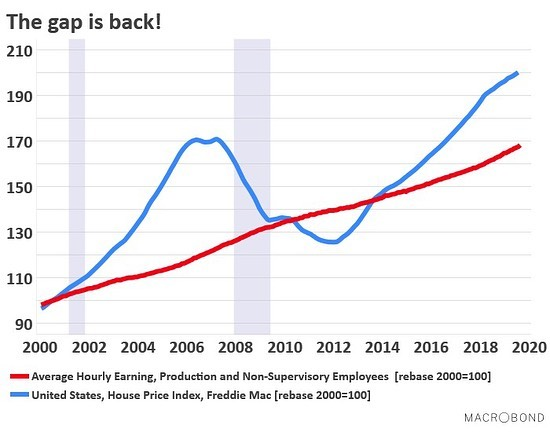
\includegraphics[height=8.5cm]{abb1}
\end{figure}

Dieser Graph wurde von Gabriel de Souza Tomitsuka mithilfe von Macrobond erstellt.
\newline

\textbf{Abbildung 2: Subprime-Kreditgeber}
\newline
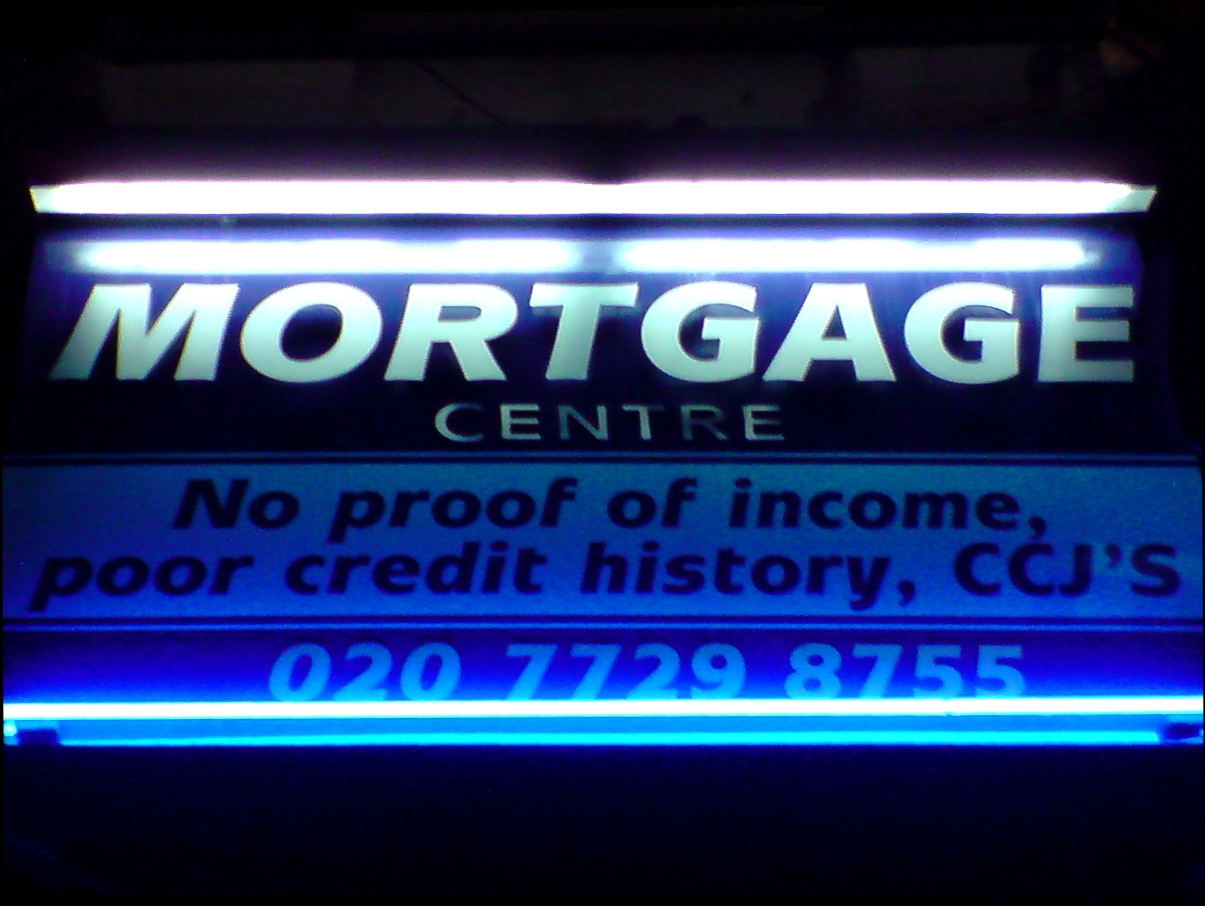
\includegraphics[height=8.5cm]{abb2}
\newpage
\textbf{Abbildung 3: Wachstum und Fall des HPIs}
\newline
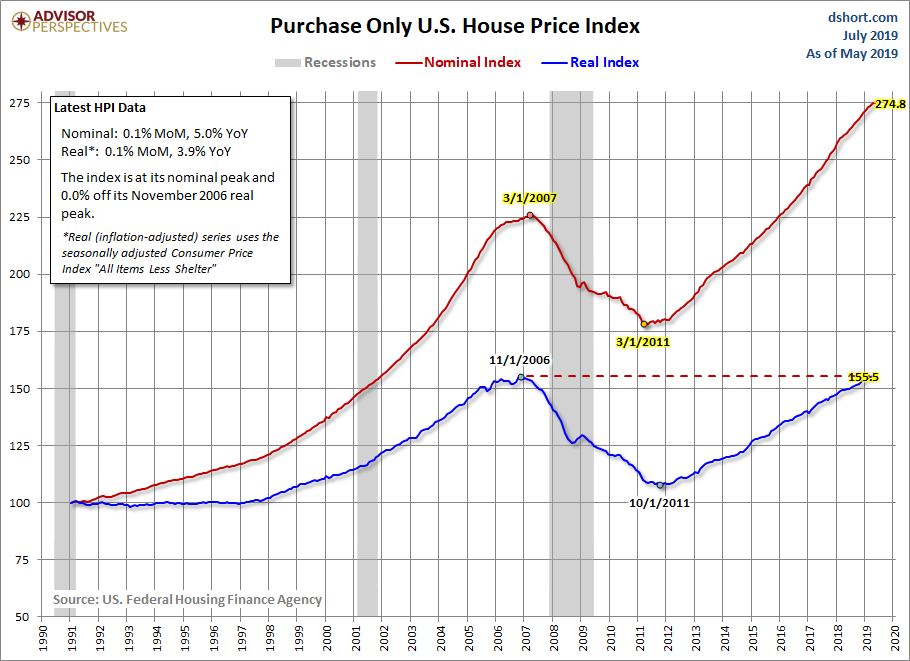
\includegraphics[width=\textwidth]{abb3}

\textbf{Abbildung 4: Preis unterschiedlicher Subprime Triple-A CDO-Tranchen, 2007-2008}
\newline
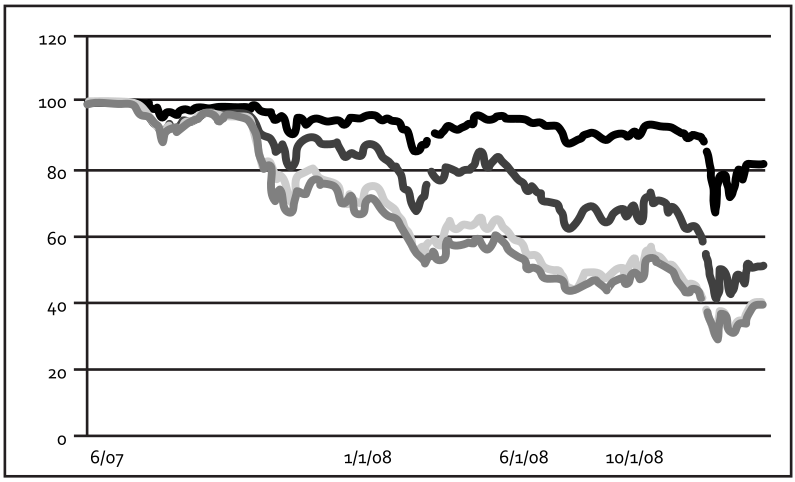
\includegraphics[width=\textwidth]{abb4}

\end{document}
http://web.mit.edu/rsi/www/pdfs/new-latex.pdf
http://web.mit.edu/rsi/www/pdfs/bibtex-format.pdf
http://www.ir.rochelleterman.com/sites/default/files/Helleiner%202011.pdf
Quelle 1: https://www.federalreserve.gov/econresdata/releases/mortoutstand/mortoutstand20090331.htm
Quelle 2: https://web.archive.org/web/20090419051155/http://www.sifma.org/uploadedFiles/Research/Statistics/SIFMA_USBondMarketOutstanding.pdf
Quelle 3: https://fraser.stlouisfed.org/timeline/financial-crisis
Quelle 4 (Doss, 2007): https://www.wsj.com/articles/SB116775515272364964
Quelle 5 (Creswell \& Bajaj, 2007): https://www.nytimes.com/2007/04/03/business/03lend.html
https://academic.oup.com/cje/article/33/4/563/1730705
GS: https://www.goldmansachs.com/insights/pages/learning-from-a-century-us-recessions/report.pdf
Buffett: https://www.youtube.com/watch?v=MQcPC31KRqA
Dimon: https://www.youtube.com/watch?v=QE3QwTA5ujE
Dimon text: https://www.jpmorganchase.com/corporate/investor-relations/document/annualreport-2018.pdf
EU: https://europa.eu/rapid/press-release_MEMO-08-123_en.htm?locale=en
ä \"a
ö \"o
ü \"u
ß
(28.09.19)
Ap. 1: mit Macro Bond selbst erstellt
Ap. 2: https://commons.wikimedia.org/wiki/File:P060708_22.03-02-retouched.jpg
Ap. 3: https://www.advisorperspectives.com/images/content_image/data/6c/6c77ccb14b1810a345ed768e3f8d5272.png
Ab. 4:
Ap. 5: https://upload.wikimedia.org/wikipedia/commons/4/4f/Einlagefazilit%C3%A4t.PNG
Ap. 6: https://wits.worldbank.org/CountryProfile/en/Country/USA/Year/2009/Summarytext
Von Alex1011 - Eigenes Werk, data from Deutsche Bundesbank, CC BY-SA 3.0, https://commons.wikimedia.org/w/index.php?curid=10648268